\section{Praktijk: neural network}

\subsection{Inleiding}
Met de kennis die we hebben opgedaan bij het maken van het theorieverslag gaan we zelf een tweede praktijkopdracht uitvoeren. We dagen onszelf uit tot het maken van een computerprogramma dat de volgende vraag beantwoordt: \textit{welke onderdelen zijn nodig voor een zelflerend computersysteem, in de vorm van een door ons ontworpen computerprogramma, dat in staat is afbeeldingen te classificeren binnen vastgestelde categorie\"en met een precisie van meer dan 80 procent?}

\subsection{Werkwijze}
Voordat we kunnen beginnen aan het ontwerp van het systeem, moeten we eerst duidelijk maken wat we precies willen bereiken en hoe we dat willen bereiken. We moesten eerst een aantal vragen beantwoorden:\\
\begin{itemize}  
\item\textbf{Welke afbeeldingen gaan we proberen te classificeren?}\\
We gaan proberen handgeschreven cijfers te classificeren. We gebruiken hiervoor de MNIST dataset \cite{MNIST}. Dit is een dataset van een groot aantal afbeeldingen van handgeschreven cijfers met het bijbehorende label. De afbeeldingen zijn elk 28 x 28 pixels groot. Deze dataset is erg geschikt om machine learning op toe te passen.
\item\textbf{Welk algoritme gebruiken we voor het classificeren van de afbeeldingen?}\\
Wij gebruiken een neural network (zie \ref{fig:ArtificialNeuralNetworks}) om deze afbeeldingen te classificeren. Het scheen ons toe dat dit het beste algoritme is voor het classificeren van afbeeldingen. Er zijn 28 * 28 = 784 input neurons en 10 output neurons. We kiezen ervoor om \'e\'en hidden layer te maken.
\item\textbf{Welke manier van leren gebruiken we voor het verbeteren voor het algoritme?}\\
We gaan gebruik maken van gradient descent (\ref{fig:GradientDescent}).
\end{itemize}

\subsection{Netwerk}
Het aantal input neurons en het aantal output neurons staat vast (respectievelijk 784 en 10). Het aantal hidden neurons kunnen we zelf bepalen. Ook moet aan elke laag nog een bias toegevoegd worden (\ref{fig:Bias}). Zoals uitgelegd in \ref{fig:ActivationFunction} moeten we ook een \textit{activation function} kiezen. Hiervoor gebruiken we een sigmoid function (zie figuur \ref{fig:sigmoid-function}). De lagen zijn onderling volledig verbonden. Elke verbinding heeft zijn eigen weging die op het begin naar een willekeurige waarde wordt gezet.

\begin{figure}[H]
	\begin{align*}
	   f(x) = \frac{1}{1 + e^{-u}}
	\end{align*}
	\caption{De sigmoid function}
\end{figure}

\begin{figure}[H]
  \centering
    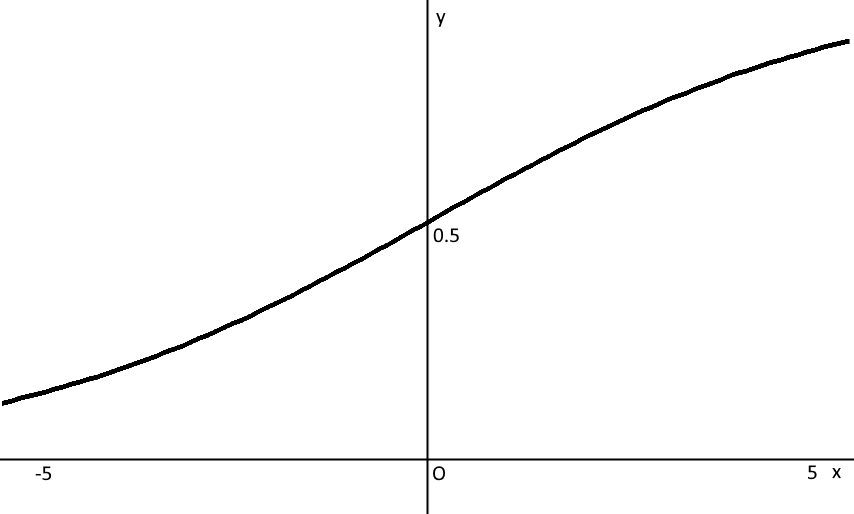
\includegraphics[width=0.5\textwidth]{sigmoid.png}
  \caption{De grafiek van de sigmoid function}
  \label{fig:sigmoid-function}
\end{figure}


\subsection{Gradient descent}
Nu we een werkend netwerk hebben kunnen we naar het belangrijkste deel kijken: het vinden van de juiste wegingen voor de neurons. Zoals gezegd gaan we dit doen door middel van gradient descent.
Wat we gaan doen is: \textit{het bepalen van de afgeleide van de cost function relatief tot de te veranderen variable.}

\begin{figure}[H]
  \centering
    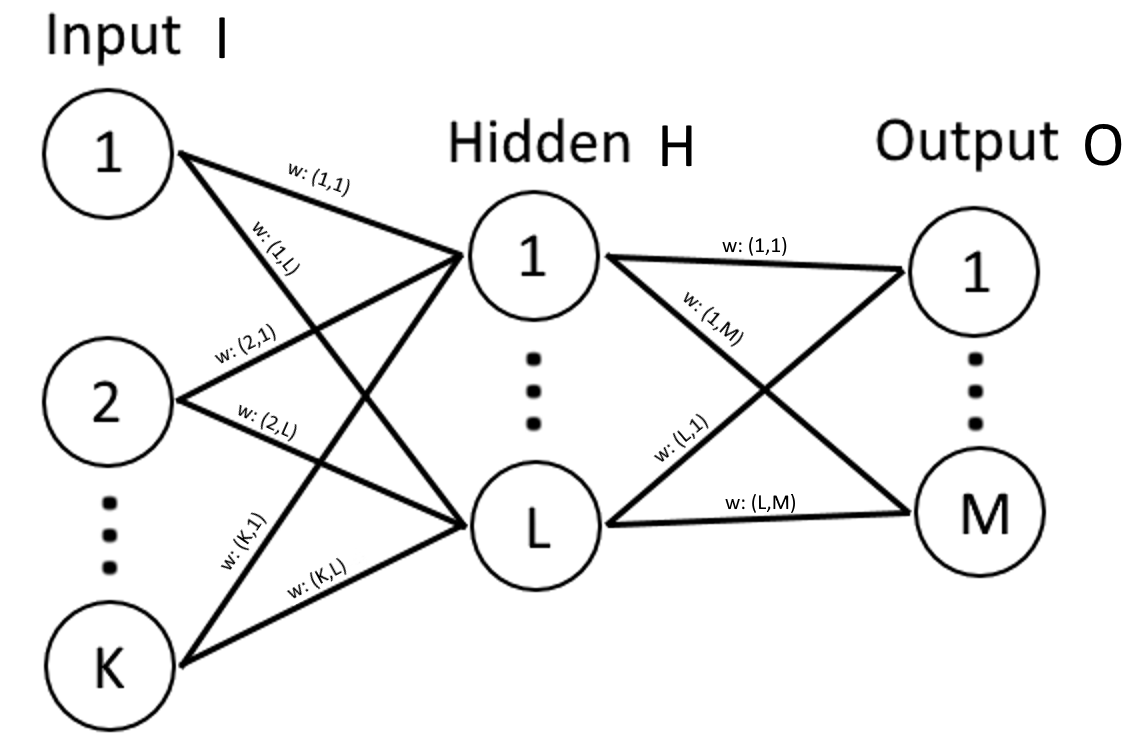
\includegraphics[width=\textwidth]{NeuralNetworkWeights.png}
  \caption{Een neural network met aangegeven weights}
  \label{fig:NeuralNetworkWeights}
\end{figure}

De cost function is:

$$ C(x) = \frac{1}{2}\sum_{m=1}^{M}(y_{m}-t_{m})^2 $$

Let op dat $\frac{1}{2}$ gewoon wordt toegevoegd om later makkelijker de afgeleide te kunnen bepalen. We moeten ook de afgeleide van de sigmoid function weten, deze is gelukkig erg simpel, namelijk:

$$ f'(x) = f(u)(1-f(u))) $$

Wat we nu doen is het bepalen van de afgeleide van de cost function relatief tot de weging van de hidden neurons naar de output neurons ($w_{ho}$). Om tot dit resultaat te komen, moeten we een aantal keer de kettingregel toepassen:

\begin{align*}
	c'(x) &= (O_{m}-t_{m}) * O' \\
	O' &= O_{m}(1-O_{m}) * H_{l} \\
	c'(x) &= (O_{m}-t_{m}) * O_{m}(1-O_{m})*H_{l}
\end{align*}

Nu we de afgeleide berekend hebben, kunnen we de weight een beetje in de goede richting verplaatsen. Hierin staat $\eta$ voor de learning rate (\ref{fig:LearningRate}).

$$ w_{lm} = w_{lm} - \eta *(O_{m}-t_{m}) * O_{m}(1-O_{m})*H_{l} $$

Om de afgeleide van de cost function te bepalen relatief tot de weging van de de input neurons naar de hidden neurons moeten we nog een aantal keer de kettingregel toepassen:

\begin{align*}
	C'(x) &= \sum_{m=1}^{M}[(O_{m}-t_{m}) * O'] \\
	O' &= O_{m}(1-O_{m}) * H_{l} * H' \\
	H' &= H_{l}(1-H_{l})*I_{k}\\
	C'(x) &= \sum_{m=1}^{M}[(O_{m}-t_{m}) * O_{m}(1-O_{m})*w_{ho}]*H_{l}(1-H_{l})*I_{k}
\end{align*}



De weging $w_{lm}$ wordt dan:

$$ w_{lm} = w_{lm} - \eta *\sum_{m=1}^{M}[(O_{m}-t_{m}) * O_{m}(1-O_{m})*w_{ij}]*H_{l}(1-H_{l})*I_{k} $$

\subsection{Het programma}
Bij het opstarten van het programma verschijnt een scherm waarin de beginwaardes van het neural network bepaald kunnen worden en het probleem gekozen kan worden. Als je met de muis op een onderdeel staat, verschijnt er meer informatie over het desbetreffende onderdeel. Verder is een weergave te zien van het neural network. Hierin geeft een rode verbinding een negatieve weging aan, en een blauwe verbinding een positieve weging aan.
Om uit te testen of het programma goed functioneert, hebben we eerst een simpel probleem uitgetest: XOR. Het doel van een XOR poort is als volgt: als \'e\'en van beide input waardes $"1"$ is, moet het antwoord $"1"$ worden, anders $"0"$. Na even trainen leert het neural network dit probleem op te lossen! Dit betekent dat het programma goed functioneert, dus kunnen we naar het \textit{echte} probleem.

\begin{figure}[H]
  \centering
    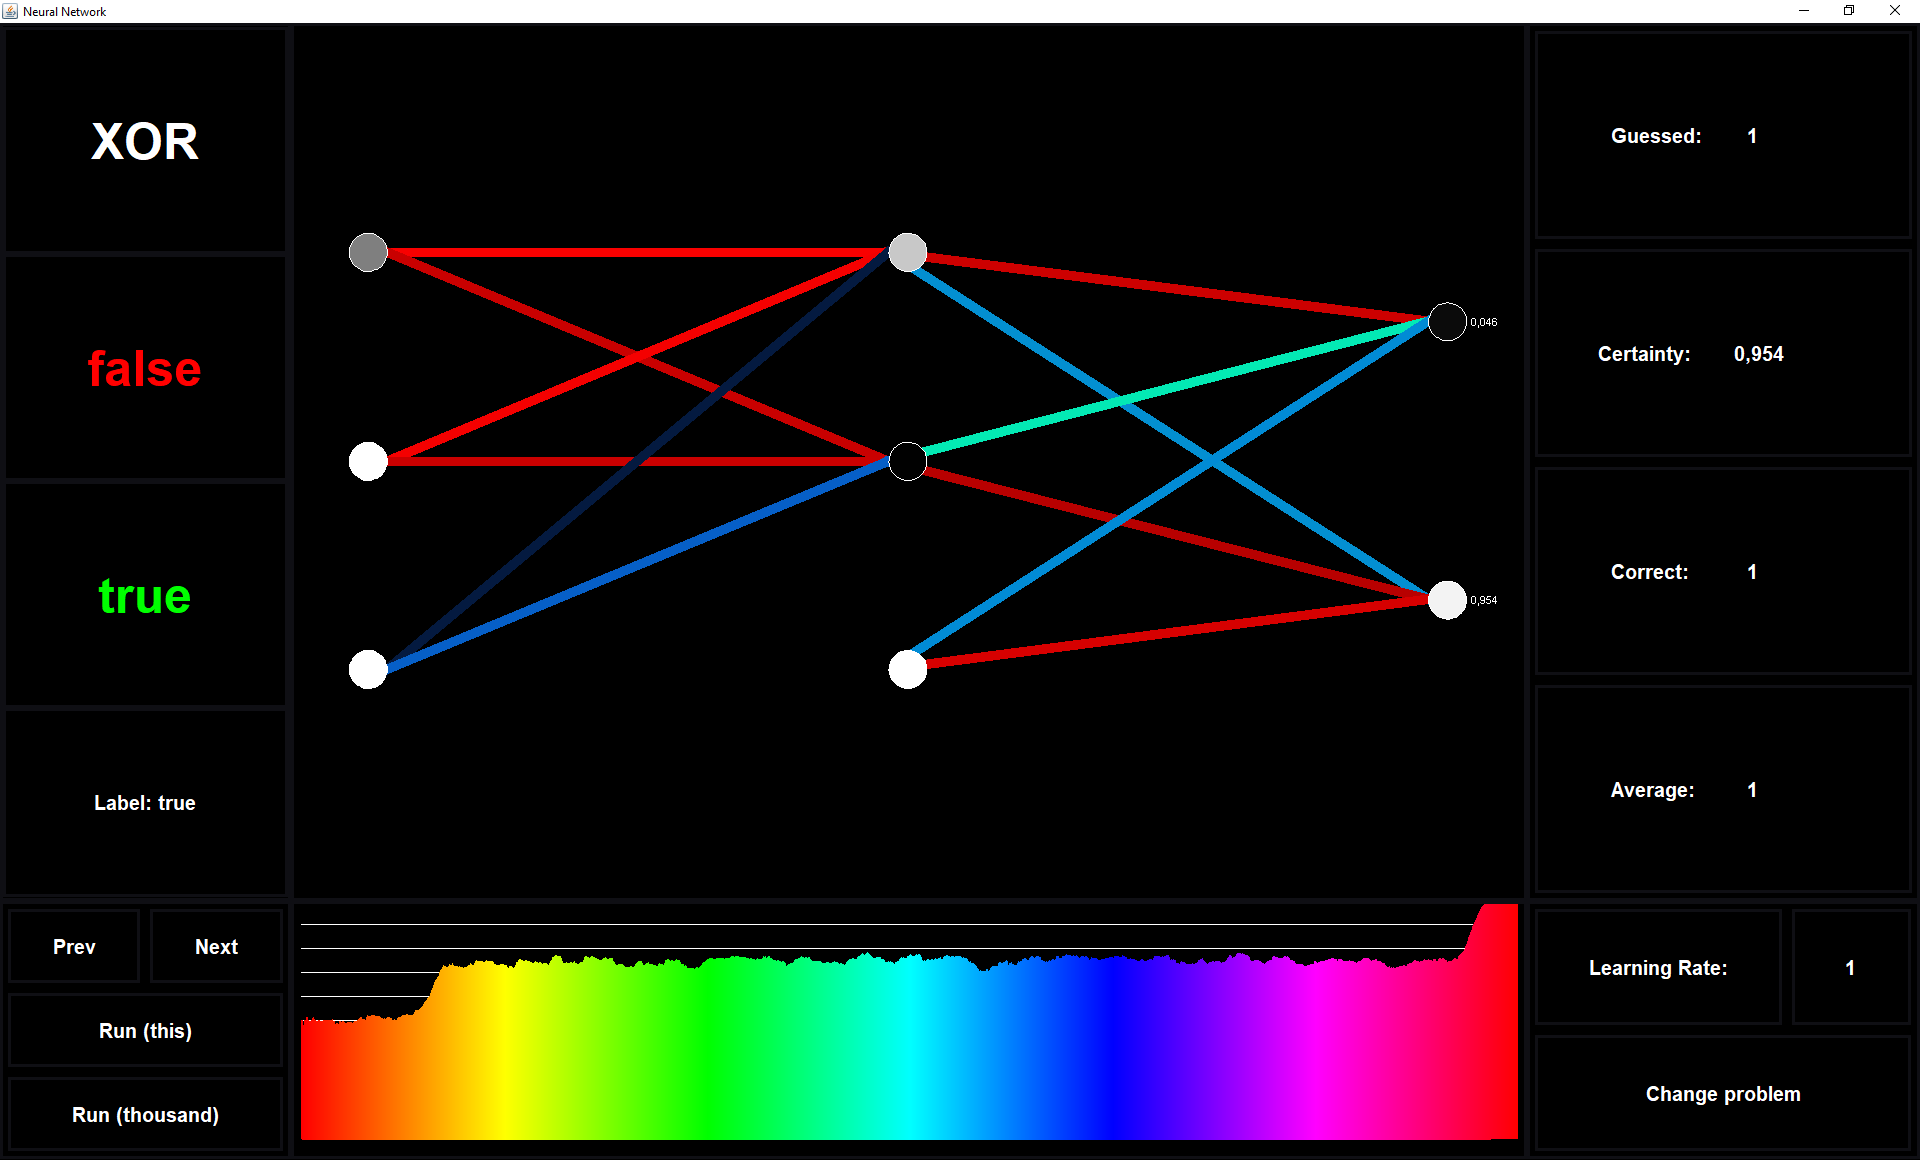
\includegraphics[width=\textwidth]{NeuralNetworkXOR.png}
  \caption{Het door ons geschreven neural network programma dat zelf heeft geleerd XOR-probleem op te lossen}
  \label{fig:NNXOR}
\end{figure}

\subsection{Resultaten}
De prestaties van het neural network worden door een aantal variablen bee\"invloed:

\begin{itemize}
  \item Het aantal hidden neurons
  \item De learnig rate
  \item Het aantal training plaatjes
\end{itemize}

In figuur \ref{fig:NNXOR} is te zien welk effect het veranderen van de variablen heeft op de prestaties van het netwerk.

\begin{figure}[H]
  \centering
    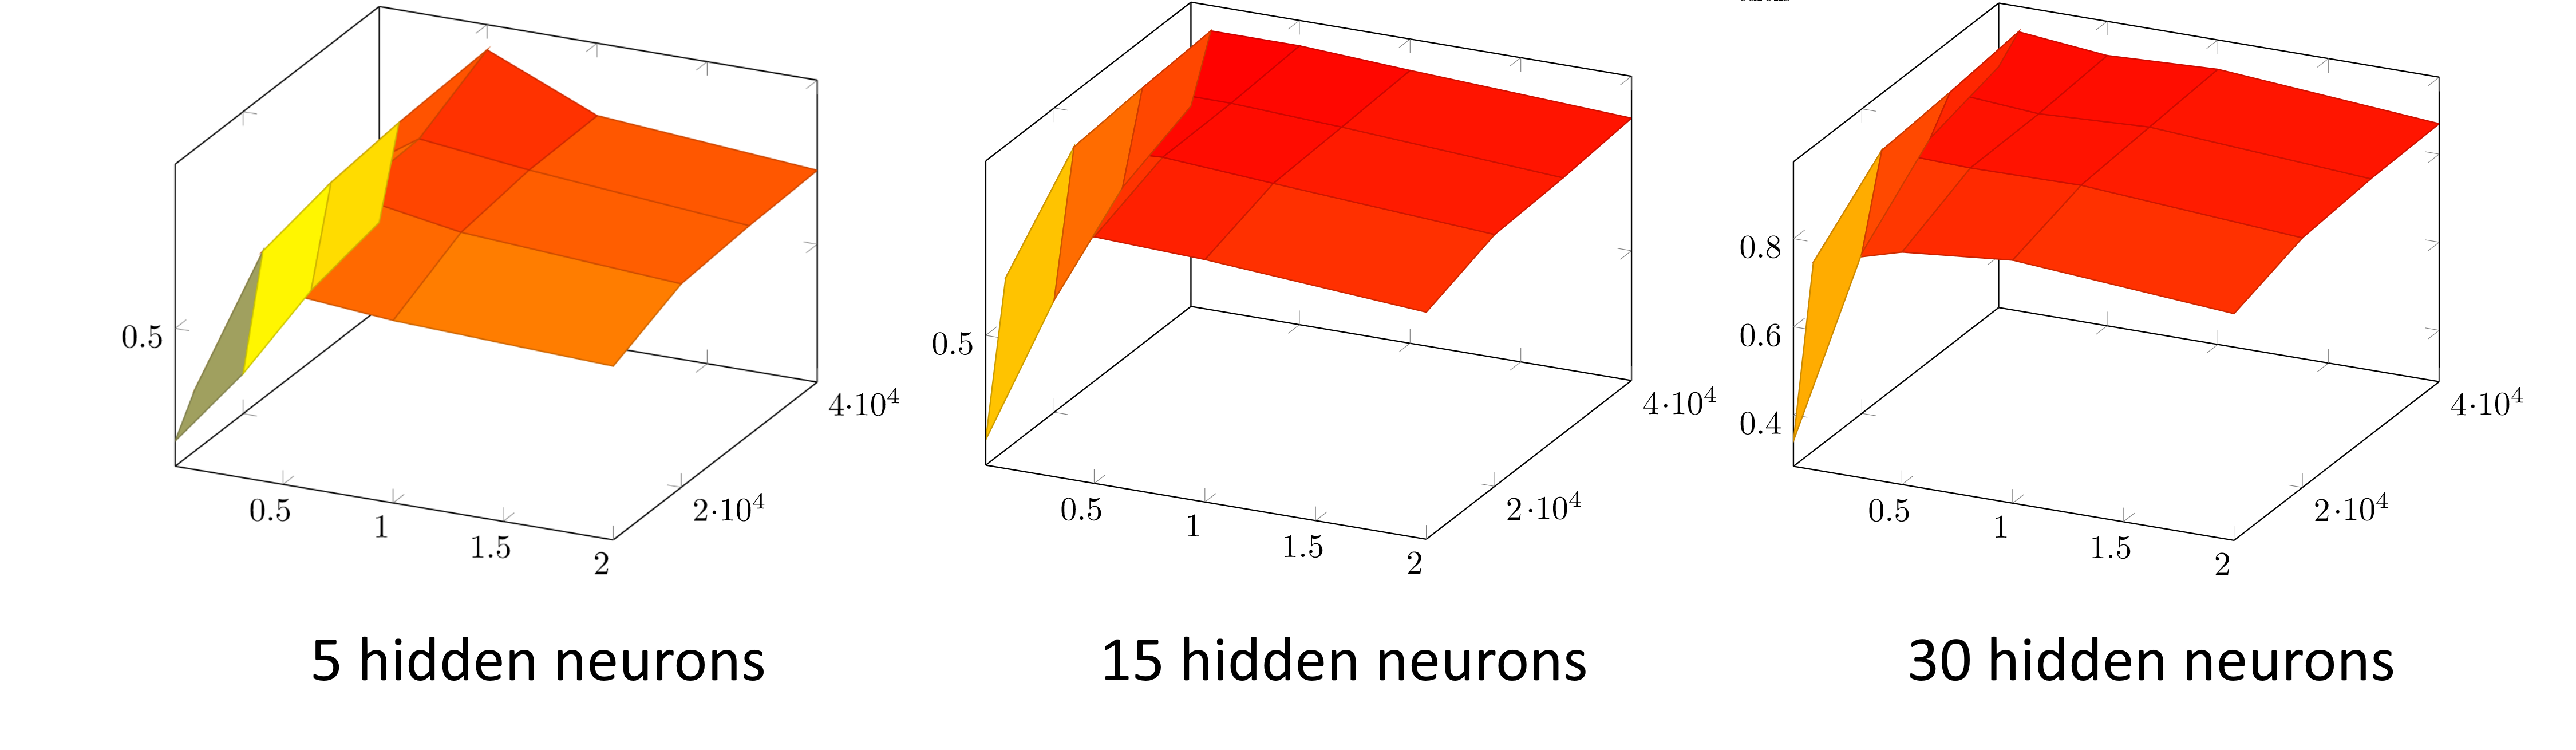
\includegraphics[width=\textwidth]{NeuralNetworkDigitRecognitionResults.png}
  \caption{De resultaten van ons neural network.
  De y-as duidt de prestatie van het netwerk aan.
  De x-as duidt de de learning rate aan.
  De z-as duidt het aantal plaatjes aan.}
  \label{fig:NNXOR}
\end{figure}

\begin{figure}[H]
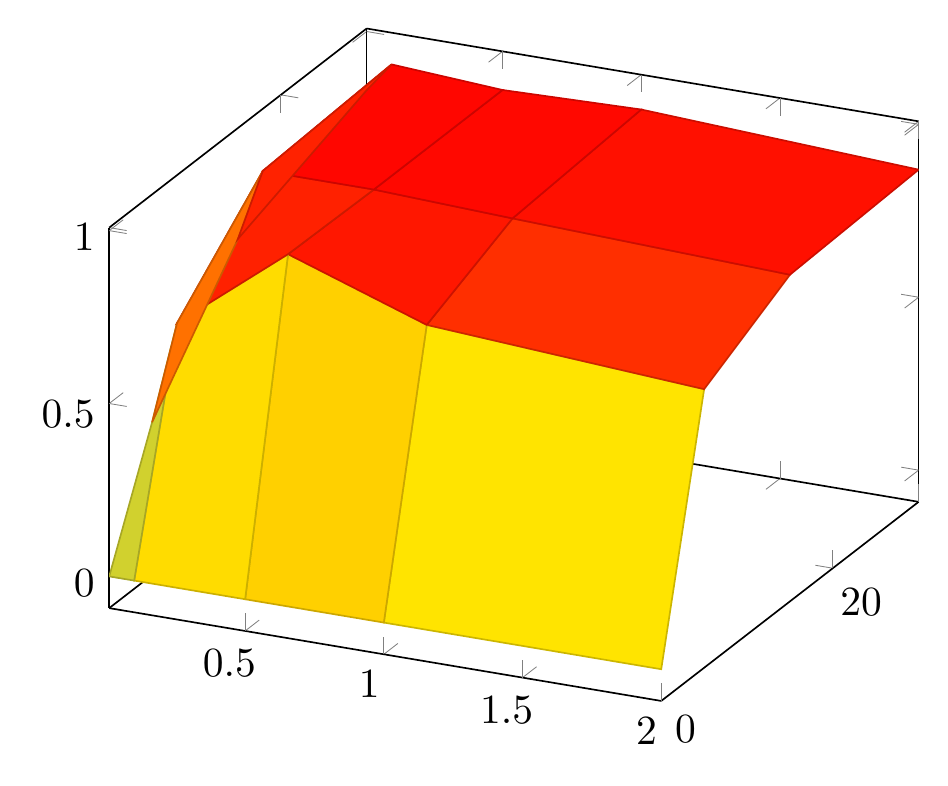
\begin{tikzpicture}[scale=1.5]
\begin{axis} 
\addplot3[surf] coordinates{
(0.01,0,0) (0.01,5,0.350) (0.01,15,0.688) (0.01,30,0.830) 

(0.1,0,0) (0.1,5,0.649) (0.1,15,0.897) (0.1,30,0.917) 

(0.5,0,0) (0.5,5,0.902) (0.5,15,0.897) (0.5,30,0.897) 

(1,0,0) (1,5,0.765) (1,15,0.881) (1,30,0.908)

(2,0,0) (2,5,0.714) (2,15,0.853) (2,30,0.869)

};

\end{axis}
\end{tikzpicture}
\caption{De resultaten van ons neural network getraind op \textbf{40000} afbeeldingen. 
De y-as duidt de prestatie van het netwerk aan. 
De x-as duidt de de learning rate aan. 
De z-as duidt het aantal hidden neurons aan.}
\end{figure}

Het hoogst behaalde resultaat is een nauwkeurigheid van 91,7\%, bij een learning rate van 0,1 en 30 hidden neurons getraind op 40000 afbeeldingen.

\subsection{Conclusie}
E\'en manier voor het maken van een computerprogramma dat in staat is afbeeldingen te categoriseren, is door gebruik te maken van een neural network dat verbeterd wordt door middel van gradient descent.
